\sectionlink{序論}

対称性の構造に基づく有効場理論（effective field theory; EFT）のアプローチは、低エネルギーのダイナミクスに普遍的な枠組みを与える~\cite{Manohar:1996cq}。
特に、対称性が破れた相のダイナミクスに適用すると非常に強力である。この相の低エネルギーのダイナミクスは、自発的に破れた対称性に伴う質量のない Nambu-Goldstone（NG）モードによって支配される。
EFT はもともと高エネルギー素粒子物理の文脈で発展したが~\cite{Coleman:1969sm,Callan:1969sn,Weinberg:1978kz}、その適用範囲は物性物理や素粒子物理から宇宙論まで、物理学のほぼすべての分野に及ぶ。
さらに、近年の応用は従来の物理学の対象を越え、例えば魚や鳥の群れのようなアクティブマター~\cite{TonerTu1,TonerTu2}にまで広がりつつある。



\medskip
EFT アプローチのさまざまな応用の中で、近年精力的に研究されている興味深い方向の一つが、開放系の実時間非平衡ダイナミクスへの応用である。そこでは、関心のあるダイナミクスが、環境に由来するノイズと散逸の影響を受ける。
最もよく知られた例は、散逸とゆらぎの両方の効果が現れる散逸的（揺動）流体力学である~\cite{Grozdanov:2013dba,Haehl:2015uoc,Crossley:2015evo,Glorioso:2017fpd,Jensen:2017kzi,Haehl:2018lcu,Jensen:2018hse}。
散逸流体力学では、保存電荷密度とそれに伴う流体力学的モードだけに注目する。これは、それ以外のすべての高エネルギーモードが環境の役割を果たすことを意味する。
さらに、保存則の破れを流体力学の方程式に取り入れることで、アクティブマターの集団的な振る舞いを記述できる（総説については文献~\cite{RevModPhys.85.1143}およびその引用文献を参照）。
もう一つの典型例は宇宙論である。宇宙論では、宇宙論的地平線の外側の自由度を観測できず、地平線の内側のダイナミクスを議論する際には、それらの自由度が環境の役割を果たす。
また、高エネルギー理論に基づくインフレーションのシナリオでは、インフラトンと重力子は一般に、直接調べることのできない質量を持つ場と結合している~\cite{Chen:2009zp,Baumann:2011nk,Noumi:2012vr,Arkani-Hamed:2015bza}。このような隠れたセクターも、やはり環境の役割を果たす。
これらの幅広い例から分かるように、開放系という見方は自然界のさまざまな系に共通する。
それにもかかわらず、確立された EFT の観点から非平衡開放系に注目し始めたのは、ごく最近のことである。

\medskip
本論文では、開放系の対称性が破れた相に対する EFT アプローチを展開する。
特に、二つの具体的な応用を念頭に置き、時間並進対称性の破れに注目する。
一つは、例えば反応拡散系で起こる同期現象~\cite{Kuramoto,MoriKuramoto}や、物性系におけるある種の時間結晶~\cite{PhysRevLett.96.230602,PhysRevLett.99.140402,sieberer2016keldysh}である\footnote{
時間結晶に関する当初の素朴な提案~\cite{Wilczek:2012jt}に反して、基底状態または熱平衡状態における量子時間結晶の実現は、理論的に否定されている~\cite{Bruno:2013mva,Watanabe:2014hea,Yamamoto:2015fxa}。
しかし、本論文で議論するように、自発的対称性の破れの概念を励起状態や非平衡状態へと拡張すれば、なお実現の可能性がある。文献~\cite{Buca:2018ccq}も参照。}。
これらの系には時間的に周期的な物理的観測量が存在する。これは、連続的な時間並進対称性が離散的なものへと破れていることを意味する。
もう一つは宇宙のインフレーション~\cite{Starobinsky:1980te,Guth:1980zm,Sato:1980yn}である。そこでは、時間に依存するインフラトン背景が時間並進対称性を破り、それに対応する NG ボソンが、宇宙マイクロ波背景放射の温度ゆらぎなど、私たちの宇宙の構造の源となる（総説として、例えば文献~\cite{Baumann:2009ds,Senatore:2016aui}を参照）。
同じ対称性の破れのパターンは、クインテッセンスと呼ばれるダークエネルギーへの現象論的アプローチにも現れる~\cite{Gubitosi:2012hu}。
孤立系については、このような時間並進対称性の破れに対する EFT アプローチは、宇宙のインフレーションの文脈ですでに詳しく研究されている~\cite{Cheung:2007st}。
本論文では、散逸流体の EFT に関する最近の発展~\cite{Crossley:2015evo,Glorioso:2017fpd}を応用し、開放系におけるノイズと散逸の効果を、時間並進対称性の破れに対するこの EFT の枠組みにさらに取り入れる。


\medskip
本論文の構成は以下のとおりである。
第\ref{section:TT}節では、散逸とランダムな力の存在下にある Brown粒子という最も単純な模型を用いて、開放系に伴う二重化された時間並進対称性とその破れなどの基本概念をまず導入する。
続いて第\ref{section:ConstructingEFT}節では、Schwinger-Keldysh 形式とその対称性構造に基づいて、時間並進対称性が破れた開放系の EFT を構築する。
構築した有効 Lagrangian を用いて、Nambu-Goldstone モードの分散関係を導出する。
一般的な帰結に加えて、単一のスカラー場からなる、具体的に解析可能な簡単な紫外（UV）模型を示し、本論文の EFT における低エネルギー（Wilson）係数と UV 理論のパラメータとの関係を明らかにする。
第\ref{section:Summary}節では、まとめと今後の展望を述べる。


\sectionlink{Brown運動の時間並進対称性}
\label{section:TT} 

まず、簡単な例である Brown粒子系を解析し、開放系に伴う対称性構造を詳しく説明する。
第\ref{section:ClassicalBrownian}節では、Langevin 方程式から出発し、Martin-Siggia-Rose（MSR）経路積分形式および Fokker-Planck 形式を導入する。
第\ref{section:BrownianSymmetries}節では、この二つの形式に基づいて、二つの時間並進対称性に関連する二種類の生成子（電荷）が存在することを示し、開放系における時間並進対称性の自発的破れ（SSB）に対する、われわれの\textit{弱い}判定基準を提示する。
また、揺動散逸関係を離散対称性の帰結としてどのように取り入れられるかも説明する。
第\ref{micro:origin}節では、Schwinger-Keldysh 形式に基づき、基礎となる量子論の観点から、二重化された対称性と離散対称性の起源を議論する。
本節で述べるすべての内容は、次節の基礎となる。
MSR 形式と Schwinger-Keldysh 形式に詳しい読者は、第\ref{sec:TimeTrSym}節の末尾に示す SSB の\textit{弱い}定義を確認すれば、本節の大部分を飛ばしてもよい。


\subsectionlink{三つの等価な形式}
\label{section:ClassicalBrownian}
揺動散逸を伴う確率系（例えば流体中の Brown粒子）を記述する最も単純で直観的な方法は、\textit{Langevin 方程式}を用いることである。
しかし、確率系に内在する対称性を議論するには、Langevin 方程式はそれほど有用ではなく、これと等価な別の定式化を用いる方が役立つ。
そこで、Brown粒子に対する Langevin 方程式から出発し、古典確率系に対する二つの等価な形式、すなわち\textit{Fokker-Planck 形式}と\textit{Martin-Siggia-Rose（MSR）形式}を導入する。
量子論との類推では、これらはそれぞれ正準演算子形式と経路積分形式に対応する。

\subsubsection{Langevin 方程式}
\label{section:Langevin}
開放系の対称性構造とそれに伴う保存電荷を説明するため、不足減衰の Langevin 方程式で記述される Brown運動を考えよう。
\begin{align}
 M \ddot X_R (t) =- V'\big(X_R(t)\big) - M \gamma \dot X_R(t) +\xi (t) \,,
 \label{eq:langevin1}
\end{align}
ここで、$X_R(t)$ は質量 $M$ の Brown粒子の位置、$V'(X_R) = \dfrac{\partial V}{\partial X_R}$ はポテンシャルエネルギー $V(X_R)$ の微分、$\gamma$ は減衰係数、$\xi (t)$ は Brown粒子に作用するランダムな力を表す。
ランダムな力 $\xi(t)$ は、次の Gaussian 白色ノイズで与えられる。
\begin{equation} 
 \langle \xi(t) \rangle_\xi  = 0 , \quad 
  \langle \xi(t)\xi(t')\rangle_\xi 
  = A \,\delta(t-t')\,,
  \label{eq:noise}
\end{equation}
ここで、ノイズ平均 $\langle \mathcal{O}(\xi) \rangle_\xi$ を次のように導入した。
\begin{equation}
 \langle \mathcal{O}(\xi) \rangle_\xi 
  \equiv \int \mathcal{D} \xi
  \mathcal P[\xi] \mathcal{O} (\xi) 
  \quad \mathrm{with} \quad 
  \mathcal P[\xi] \equiv \exp \left[ - \frac{1}{2A} \int dt\, \xi^2(t) \right].
  \label{eq:NoiseAvg}
\end{equation}
揺動散逸関係（fluctuation-dissipation relation; FDR）が成り立つ場合には、熱平衡にある周囲の流体の温度を $T$ として、$A= 2 M \gamma T$ となる。
ただし、より一般的な状況を考えるため、以下の議論では $A$ を一般の定数のままとする。
式\eqref{eq:langevin1}と式\eqref{eq:noise}は時間に陽に依存しないため、この系は時間並進対称性を持つ。言い換えると、式\eqref{eq:langevin1}は $X_R(t)\to X'_R(t)=X_R(t+\epsilon)$ および $\xi(t)\to \xi'(t)=\xi(t+\epsilon)$ の下で共変である。
ここで、\textit{「この時間並進対称性に伴う保存電荷は何か」}という自然な疑問が生じる。
明らかに、それは Brown粒子のエネルギーではない。ノイズと散逸が存在するため、そのエネルギーは保存しないからである。
\begin{align}
 \frac{d}{dt}\left[\frac{1}{2} M \dot X^2_R + V \big(X_R \big) \right] 
 = - M \gamma \dot X^2_R + \dot X_R \xi \neq 0 . \,\label{consviolgv}
\end{align}
この Brown粒子のエネルギーが時間並進を生成しないことを示すのも有益である。
そのために、運動量 $P_R$ を導入し、式\eqref{eq:langevin1}を次のように書き換えよう。
\begin{align}
 \label{eq:eom_xp}
 M \dot{X}_R  = P_R ,  \quad
 \dot{P}_R = -V' (X_R) - \gamma P_R + \xi \,.
\end{align}
Brown粒子のエネルギー $H_R$ を
\begin{align}
 H_R = \frac{P^2_R}{2M} + V(X_R) \,,
\end{align}
で導入すると、運動方程式は次のように書き換えられる。
\begin{align}
 \dot{X}_R=\frac{\partial H_R}{\partial P_R} 
 \,,
 \quad
 \dot{P}_R=-\frac{\partial H_R}{\partial X_R}- \gamma P_R + \xi\, ,
 \label{eq:langevin2}
\end{align}
したがって、$\dot{P}_R \neq \{P_R, H_R \}_{PB}$ である。ここで、$\{A,B\}_{PB}$ は Poisson 括弧である。
ノイズも散逸もなければ、$(X_R,P_R)$ を一組の正準変数とみなし、粒子のエネルギー $H_R$ を、この系の時間並進を正しく生成する Hamiltonian と同一視できる。
しかし、散逸系ではそうはいかない。
これが、単一の正準変数対によって Brown運動を記述する際の主な障害である。
また、この定式化では、時間並進対称性に伴う保存電荷が何であるかも、まだ明らかでない。

\subsubsection{Martin-Siggia-Rose 形式}
\label{section:lmsrfp}
上記の時間並進対称性の生成子を特定するには、別の等価な形式、すなわち Martin-Siggia-Rose（MSR）経路積分形式~\cite{PhysRevA.8.423,Janssen1976,PhysRevB.18.4913}と Fokker-Planck（演算子）形式を用いると便利である。
まず Langevin 方程式から出発して、MSR 形式を導入する。

量子論における通常の経路積分形式と同様に、MSR 形式で注目するのは相関関数の集合である。すなわち、次の量に関心がある。
\begin{equation}
 \langle \mathcal{O}[X_R,P_R] \rangle_\xi 
  \equiv \int \mathcal{D} \xi \mathcal P[\xi] \mathcal{O}[X_\xi,P_\xi], 
  \label{eq:correlation}
\end{equation}
ここで、$\{X_\xi(t_n), P_\xi(t_n)\}$ は Langevin 方程式\eqref{eq:langevin2}の解の集合を表し、$\mathcal P[\xi]$ は式\eqref{eq:NoiseAvg}で定義されている。
例えば $\mathcal{O}[X_R,P_R] = X_R(t_1) X_R(t_2) \cdots X_R(t_n)$ と選べば、これは Brown粒子の位置の $n$ 点関数を与える。この関数は、考えている確率過程の基本的な情報を含む。
次に、恒等式 $1 = \displaystyle{\int} \mathcal{D} X_R \mathcal{D} P_R \delta (X_R - X_\xi ) \delta (P_R - P_\xi )$ を挿入し、$\{X_\xi (t_n), P_\xi(t_n)\}$ を積分変数 $\{X_R(t_n), P_R(t_n)\}$ に置き換えると、式\eqref{eq:correlation}を次のように計算できる。
\begin{equation}
 \begin{split}
  \langle \mathcal{O}[X_R ,P_R] \rangle_\xi
  &= \int \mathcal{D} X_R  \mathcal{D} P_R \mathcal{D} \xi 
  \delta (X_R - X_\xi)  \delta (P_R - P_\xi) \mathcal P[\xi]
  \mathcal{O}[X_R,P_R] \\
  &= \int \mathcal{D} X_R \mathcal{D} P_R  J 
  \big\langle \delta (\mathrm{EoM}_{X_\xi}) \delta (\mathrm{EoM}_{P_\xi} )
  \big\rangle_\xi 
  \mathcal{O}[X_R,P_R] .
  \label{eq:2.9}
   \end{split}
\end{equation}
ここでは、デルタ汎関数を、次のように定義される運動方程式 $\mathrm{EoM}_{X_\xi, P_\xi}$ を用いて書き換えた。
\begin{equation}
 \mathrm{EoM}_{X_\xi}
 \equiv 
   \dot{X}_R - \frac{P_R}{M} , \quad
   \mathrm{EoM}_{P_\xi}
 \equiv 
  - \dot{P}_R + \big[ - V'(X_R) - \gamma P_R + \xi \big],
\end{equation}
この書き換えにより、Jacobian $J \equiv \det \left| \dfrac{\delta (\mathrm{EoM}_{X_\xi})}{\delta X_R} \right| \det \left| \dfrac{\delta (\mathrm{EoM}_{P_\xi})}{\delta P_R} \right|$ が現れる。
一般には、この Jacobian は、例えばループ計算を行う際に重要な役割を果たしうる。
しかし、各運動方程式には、それぞれ $X_R$ および $P_R$ について非線形な項が含まれていないので、Jacobian の部分を考慮する必要はない。
デルタ汎関数の Fourier 表示
\begin{align}
 \delta(\mathrm{EoM}_{X_\xi})
 &\propto
 \int \mathcal{D}P_A 
 \exp\left[ i\int dt P_A \big( \mathrm{EoM}_{X_\xi} \big) \right],\\
 \delta(\mathrm{EoM}_{P_\xi})
 &\propto \int \mathcal{D} X_A 
 \exp \left[ i\int dt X_A \big( \mathrm{EoM}_{P_\xi} \big) \right] ,
\end{align}
を用いれば、Gaussian ノイズの積分を実行でき、次の結果を得る。
\begin{equation}
 \begin{split}
  \langle \mathcal{O}[X_R,P_R] \rangle_\xi
  &= \mathcal N \int \mathcal{D} X_R \mathcal{D} X_A \mathcal{D} P_R  \mathcal{D} P_A J
  \exp \Big( iS_{\mathrm{MSR}} [X_R,X_A,P_R,P_A] \Big)
  \mathcal{O}[X_R,P_R]
 \end{split}
\end{equation}
ここで $\mathcal N$ は全体にかかる定数であり、位相空間の MSR 有効作用を次のように導入した。
\begin{align}
 iS_{\mathrm{MSR}}[X_R,X_A,P_R,P_A] 
 &=\int dt\, \left[  i P_A \left( \dot{X}_R - \frac{P_R}{M} \right) 
 - i X_A \big(\dot P_R+ V'(X_R) + \gamma P_R  \big)
 - \frac{A}{2}X_A^2\right].
 \label{eq:MSR1}
 \end{align}
さらに、運動量 $P_R$ と $P_A$ を積分消去すると、Brown粒子に対する配位空間の MSR 有効作用が得られる。
\begin{align}
 iS_{\rm MSR}[X_{R},X_{A}]=\int dt\, 
 \Big[  -i X_A \big( M\ddot{X}_R + M \gamma\dot{X}_{R} + V'(X_{R})
  \big)  - \frac{A}{2}X_A^2 \Big]. \label{eq:MSR2}
\end{align}
このように、古典確率系である Brown運動は、もとの変数 $X_R(t)$ と、応答場または先進変数として知られる補助変数 $X_A(t)$ に関する経路積分で書き表される。
これで時間並進不変な作用が得られたので、時間並進対称性に伴う対称性の性質を議論するのは容易である。
ただし、対称性の議論に移る前に、次の小節で、もう一つの有用な形式である Fokker-Planck 形式を導入する。



\subsubsection{Fokker-Planck 形式}
次に、対称性の性質を議論するため、対応する演算子形式である Fokker-Planck 形式へ進もう。
この形式では、次式で定義される確率分布関数 $\Pcal[X_R,P_R;t]$ が中心的な役割を果たす。
\begin{equation}
 \Pcal[X_R,P_R;t] 
  \equiv 
  \big\langle \delta \big(X_R - X_\xi (t) \big) 
  \delta \big( P_R - P_\xi(t)  \big) \big\rangle_\xi,
\end{equation}
ここで、確率変数 $\{X_\xi (t),P_\xi (t)\}$ は Langevin 方程式\eqref{eq:langevin2}に従う。
Langevin 方程式を用いて、この確率分布の時間微分を注意深く計算すると、次の Fokker-Planck 方程式が得られる\footnote{
正確には、不足減衰の Langevin 方程式を考えているため、これは Fokker-Planck 方程式として知られる方程式ではなく、Kramers 方程式として知られる方程式である。}。
\begin{equation}
 \begin{split}
  \frac{\partial \Pcal}{\partial t} 
  = \left[ -\frac{P_R}{M} \frac{\partial}{\partial X_R} 
  + \frac{\partial}{\partial P_R} 
  \left( \frac{\partial V}{\partial X_R}  + \gamma P_R \right)
  + \frac{\partial^2}{\partial P^2_R} \frac{A}{2} \right] 
  \Pcal .
 \end{split}
 \label{eq:FP1}
\end{equation}
量子論の演算子形式との類似を明確にするため、次の演算子の組を定義する。
\begin{equation}
 \hat{X}_R \equiv X_R, \quad 
  \hat{P}_A \equiv \frac{1}{i}\dfrac{\partial}{\partial X_R}
  \quad \mathrm{and} \quad
  \hat{P}_R \equiv P_R , \quad 
  \hat{X}_A  \equiv i \dfrac{\partial}{\partial P_R} ,
\end{equation}
前半と後半の二つの演算子は、それぞれ共役変数の組をなし、したがって次の関係を満たす。
\begin{align}
 [\hat{X}_R, \hat{P}_A] = [\hat{X}_A, \hat{P}_R] = i,  
 \quad 
(\mathrm{others}) = 0  \, .
\end{align}
量子論の場合と同様に、角括弧は交換関係 $[\hat{A}, \hat{B}] \equiv \hat{A} \hat{B} - \hat{B} \hat{A}$ を表す。
これらの演算子を用いると、Fokker-Planck 方程式\eqref{eq:FP1}を、Schr\"odinger 方程式に類似した次の方程式に書き換えられる。
\begin{equation}
 \partial_t \Pcal [X_R,P_R;t] = - \hat{H}_A \Pcal [X_R,P_R;t]\,,\label{eq:sch}
\end{equation}
ここで、Fokker-Planck Hamiltonian $\hat{H}_A$ を次のように導入した\footnote{
別の方法として、Legendre 変換を用いれば、この Fokker-Planck Hamiltonian を MSR 形式から直接導出することもできる。}。
\begin{equation}
 \begin{split}
  \hat{H}_A 
  = \frac{i}{M} \hat{P}_R \hat{P}_A  
  + i \hat{X}_A V'(\hat{X}_R) 
  + i\gamma \hat{X}_A \hat{P}_R
  + \frac{A}{2} \hat{X}_A^2.
 \end{split}
 \label{eq:FP2}
\end{equation}
ここでは、ノイズ振幅 $A$ と減衰係数 $\gamma$ の $P_R$ 依存性を無視している。
確率分布関数について Schr\"odinger 方程式に類似した方程式が得られたので、Fokker-Planck Hamiltonian を時間並進の生成子と考えることができる。
実際、Heisenberg 描像に類似した描像を用いて、任意の演算子 $\hOcal (t)$ の時間発展を次のように記述できる（例えば文献~\cite{Zinn1996quantum}を参照）。
\begin{equation}
 \partial_t \hOcal (t) = [\hat{H}_A, \hOcal (t)]
  \with
  \hOcal (t) = e^{ \hat{H}_A t } \hOcal e^{- \hat{H}_A t}.
  \label{eq:EoMinFP}
\end{equation}
Fokker-Planck Hamiltonian が、物理的演算子 $\{\hat{X}_{R,A}, \hat{P}_{R,A}\}$ に時間並進の生成子として正しく作用することを確認しよう。
\begin{align}
 \partial_t \hat{X}_R &= [\hat{H}_A, \hat{X}_R] = \frac{\hat{P}_R}{M} 
 \,\label{HPtrsf:1},
 \\
 \partial_t \hat{P}_R &= [\hat{H}_A, \hat{P}_R] 
 = -V'(\hat{X}_R) - \gamma \hat{P}_R + iA \hat{X}_A \,, 
 \\ 
 \partial_t \hat{X}_A &= [\hat{H}_A, \hat{X}_A] 
 = \frac{\hat{P}_A}{M} + \gamma \hat{X}_A\,,
 \\
 \partial_t \hat{P}_A &= [\hat{H}_A, \hat{P}_A] 
 = - \hat{X}_A  V''(\hat{X}_R) \,\label{HPtrsf:4},
\end{align}
これらは、MSR 作用\eqref{eq:MSR1}から従う、期待どおりの運動方程式を再現している。


\subsectionlink{Brown運動に伴う対称性}
\label{section:BrownianSymmetries}

前小節で導入した MSR 形式と Fokker-Planck 形式を用いて、Brown運動に伴う対称性と生成子を示す。
一方の対称性はゆらぎと散逸が存在すると陽に破れ、もう一方は第\ref{section:Langevin}節で提起した疑問への答えを与える。
開放系の時間並進対称性の SSB に対する\textit{弱い}定義を提示した後、揺動散逸関係の情報を含む別の離散対称性も議論する。


\subsubsection{時間並進対称性}
\label{sec:TimeTrSym}
Fokker-Planck 形式と MSR 形式の観点から、Brown粒子系の対称性構造を見てみよう。
まず、すでに述べたように、MSR 有効作用\eqref{eq:MSR2}は時間に陽に依存せず、したがって $\epsilon_R$ でラベル付けされる次の時間並進の下で不変である。
\begin{equation}
 \begin{cases}
  X_R (t) \to X_R' (t) = X_R ( t + \epsilon_R ), \\ 
  X_A (t) \to X_A' (t) = X_A ( t + \epsilon_R ).
 \end{cases}
 \label{eq:Timetr1}
\end{equation}
この不変性から、次の保存電荷が得られる。
\begin{equation}
  H_A 
  = i M\dot{X}_R \dot{X}_A + i X_A V'(X_R) + \frac{A}{2} X_A^2 ,
\end{equation}
これはまさに、配位空間で表された Fokker-Planck Hamiltonian である。
式\eqref{eq:EoMinFP}を思い出せば、Fokker-Planck 形式ではこのことを容易に理解できる。演算子の時間発展は $\hat{H}_A$ によって生成されるので、$\hat{H}_A$ は自明に保存するからである。
\begin{align}
\frac{d }{dt}\hat H_{A}=[\hat H_{A},\hat H_{A}]=0.
\end{align}
したがって、Fokker-Planck Hamiltonian $\hat H_{A}$ こそ、求めていた時間並進の保存電荷、言い換えれば生成子である。

\medskip
では、もとの Hamiltonian $H_R$ はどうだろうか。
Fokker-Planck 形式の式\eqref{HPtrsf:1}から式\eqref{HPtrsf:4}を用いれば、Brown運動のもとの Hamiltonian
\begin{align}
 \hat{H}_R=\frac{\hat{P}^2_R}{2M} + V(\hat{X}_R)\,.
\end{align}
の性質を明らかにできる。
先に述べたように、ゆらぎと散逸が存在するため、これは保存しない。
実際、Fokker-Planck Hamiltonian を用いると、次式が得られる。
\begin{align}
 \frac{d}{dt} \hat{H}_R =  [\hat{H}_A, \hat{H}_R] 
 = -\frac{\gamma}{M} \hat{P}^2_R 
 + i\frac{A}{2M} 
 \big(\hat{X}_A \hat{P}_R + \hat{P}_R \hat{X}_A \big) \,,
\end{align}
これがゼロになるのは、ノイズも散逸もない場合、すなわち $\gamma=A=0$ の場合に限られる。
$\hat H_R$ が生成する無限小変換を $\delta_{\epsilon_A} \hat{\mathcal{O}} \equiv i\epsilon_A [\hat{H}_R, \hat{\mathcal{O}}]$ と定義すると、さらに次式を得る。
\begin{align}
 \label{Hx}
 \delta_{\epsilon_A} \hat{X}_R &= i\epsilon_A[\hat{H}_R, \hat{X}_R] = 0\,,
 \\
 \delta_{\epsilon_A} \hat{P}_R &= i\epsilon_A [\hat{H}_R, \hat{P}_R] = 0\,,
 \\
 \label{Hx_A}
 \delta_{\epsilon_A} \hat{X}_A &= i\epsilon_A [\hat{H}_R, \hat{X}_A] 
 = \epsilon_A\frac{\hat{P}_R}{M} = \epsilon_A \partial_t \hat{X}_R\,,
 \\
 \delta_{\epsilon_A} \hat{P}_A &= i\epsilon_A [ \hat{H}_R, \hat{P}_A] 
 = -\epsilon_A V'(\hat{x}_R)\,.
\end{align}
特に、変数 $\hat{X}_A$ が $\hat{X}_R$ の時間微分に写されることに注意しよう。
MSR 形式の観点では、これは、MSR 有効作用\eqref{eq:MSR2}が $\epsilon_A$ でラベル付けされる次の無限小変換の下で\textit{不変でない}ことに反映されている。
\begin{equation}
 \begin{cases}
  X_R (t) \to X_R' (t) = X_R (t), \\ 
  X_A (t) \to X_A' (t) = X_A (t) + \epsilon_A \dot{X}_R .
 \end{cases}
 \label{eq:Timetr2}
\end{equation}
配位空間の作用を得るために $P_R$ と $P_A$ の積分を実行しているので、ここでは $X_R$ と $X_A$ に関する変換だけが残る。
式\eqref{eq:Timetr2}の下での変分 $\delta_{\epsilon_A} S_{\msr} \equiv S_{\msr} [X_R', X_A'] - S_{\msr} [X_R, X_A]$ は、次のようになる。
\begin{equation}
 \begin{split}
  \delta_{\epsilon_A} S_{\msr} 
  &= - \epsilon_A \int dt
  \Big[ i M \dot{X}_R \ddot{X}_R + i\dot{X}_R V'(X_R) 
  + M \gamma \dot{X}_R^2 + A X_A \dot{X}_R \Big]
  + O \big( \epsilon_A^2 \big) \\
  &= - i \epsilon_A \int dt
  \frac{d H_R}{dt} 
  -  \epsilon_A \int dt
  \Big[ M \gamma \dot{X}_R^2 + A X_A \dot{X}_R \Big]
  + O \big( \epsilon_A^2 \big) .
 \end{split}
\end{equation}
第1項は Hamiltonian の全微分であり、式\eqref{eq:Timetr2}の対称性を保つが、第2項はゆらぎと散逸が存在すると消えない。

\medskip
以上の結果をまとめると、次のようになる。
Brown粒子系のような開放系を考えると、二つの時間並進対称性が存在し、これらを $H_R$ 対称性と $H_A$ 対称性と呼ぶ。前者は陽に破れており、後者は破れていない。
それぞれに伴う保存電荷、あるいは生成子は、もとの Hamiltonian と Fokker-Planck Hamiltonian である。
この二重化された対称性構造は、Schwinger-Keldysh 形式を用いると、基礎となる量子論から自然に理解できる。この点は第\ref{micro:origin}節で見ることにする。


\medskip 
この小節の最後に、二重化された時間並進対称性の自発的破れ（SSB）を議論しよう。
詳しく述べたように、ゆらぎと散逸がゼロでないために系の Hamiltonian はもはや保存せず、一方の対称性（$H_R$ 対称性）は陽に破れている。そこで、Fokker-Planck Hamiltonian $\hat{H}_A$ が生成する、もう一方の対称性（$H_A$ 対称性）に注目する。
この対称性構造は、環境が存在することで保存則を破ることのできる開放系の顕著な特徴である\footnote{
ただし、ゆらぎと散逸があっても保存則が存在する状況があることに注意する。
そのような例の一つが、散逸流体力学の EFT である（詳しい議論は、例えば文献~\cite{Crossley:2015evo,Glorioso:2017fpd}を参照）。
この種の閉じた散逸系には保存則があるが、対応する対称性は Schwinger-Keldysh 形式の閉時間経路という性質のために破れている。
その結果、この対称性（例えば $H_R$ 対称性）は非線形に実現され、低エネルギー有効理論はある種の NG モードによって記述される。}。
開放系におけるゆらぎと散逸が小さい場合、$H_R$ 対称性を近似的な対称性と考えることができ、スプリオン場を用いて、そのような弱い開放系の有効場理論を構築できることを指摘しておこう。
本論文では、エネルギー保存（$H_R$ 対称性）を陽に破る強い開放系だけに注目し、以下の意味で $H_A$ 対称性の自発的破れを考える。

\medskip
Schr\"odinger 方程式に類似した式\eqref{eq:sch}を思い出し、確率分布 $\Pcal$ に Noether 電荷 $\hat{Q}$、ここでは Fokker-Planck Hamiltonian $\hat{H}_A$ を作用させることで、SSB に対する\textit{弱い}判定基準\footnote{
ここでは、系の真空または基底状態に関する通常の（\textit{強い}）SSB の定義と区別するため、この判定基準を\textit{弱い}と呼ぶ。
通常は、Noether 電荷、より正確には Noether 電荷と秩序変数場の交換関係を真空状態に作用させ、SSB が起こるかどうかを判定する。
ここでは真空状態を考えていないため、われわれの判定基準を\textit{弱い}と呼ぶ。
\label{footnote4}}を定める。$\hat Q \Pcal = 0$ ならば系は対称性を保ち、$\hat Q \Pcal \neq 0$ ならば SSB が起こる。
定常分布 $\Pcal_{\rm eq}$ については、次式が成り立つ。
\begin{align}
 \hat H_A \Pcal_{\rm eq} = 0.\label{nonssbeq}
\end{align}
これは、定常分布が文字どおり時間並進不変であることを意味する。
したがって、$\hat{H}_A$ の最小固有値がゼロならば、系はしばらくすると時間並進対称な相に落ち着く。
一方、一般の時間に依存する確率分布 $\Pcal$ については、次式が成り立つ。
\begin{align}
 \hat H_A \Pcal \neq 0. \label{ssbnoneq}
\end{align}
この場合、われわれの（弱い）判定基準に従えば、時間に依存する確率分布を、対称性が破れた相と解釈できる。
SSB に対するわれわれの\textit{弱い}定義をどう捉えるかにかかわらず、式\eqref{ssbnoneq}は、開放系における時間並進対称性の破れの EFT を構築する出発点を与えるという本質的な役割を果たす。
式\eqref{ssbnoneq}を、例えばスローロール近似と組み合わせると、非定常系の低エネルギーのダイナミクスは、時間に依存する背景の周りの摂動を表す Nambu-Goldstone 場の有効場理論によって記述できることが分かる\footnote{
厳密に言えば、SSB に対する弱い判定基準を用いているので、これを Nambu-Goldstone 場と呼ぶのは適切でないかもしれない。
しかし、この場は自発的に破れた対称性の下で非線形に変換するため、表現論の観点からは、通常の Nambu-Goldstone 場と同じ性質に従う。
したがって、本論文ではこれを Nambu-Goldstone 場と呼ぶ。}。


\subsubsection{動的 KMS 対称性}
\label{subsec:KMS_B}

この小節では、離散対称性を用いて、配位空間の MSR 有効作用に揺動散逸関係（FDR）を組み込む方法について述べる。
式\eqref{eq:NoiseAvg}の直後に述べたように、詳細釣り合い条件に従う系では、FDR $A= 2M \gamma T$ が成り立つ。
さらに、系が初期時刻（$ t = - \infty$）に熱平衡状態にある場合には、逆温度 $\beta = 1/T$ の平衡確率分布 $\mathcal P_{\mathrm{eq}} \propto e^{- \beta H_R (t = - \infty)}$ によって平均を取る。
このとき、全体の MSR 有効作用は次のようになる。
\begin{align}
\nonumber
 &iS_{\rm MSR} [X_{R},X_{A}]  - \beta H_R (t=-\infty)
 \\
& = \int_{-\infty}^{\infty} dt\, 
 \Big[  -i X_A \big( M\ddot{X}_R + M \gamma\dot{X}_{R} + V'(X_{R})
 \big) - M \gamma T X_A^2 \Big] 
 - \beta H_R (t=-\infty), \label{eq:MSR+H}
\end{align}
ここでは、積分領域を明示した。
EFT の観点から見ると、この場合には低エネルギー（Wilson）係数の間に非自明な関係が存在する。
その結果、次の変換で生成される、動的 KMS（Kubo-Martin-Schwinger）対称性~\cite{Aron,Glorioso:2017fpd,Aron2,Sieberer:2015hba}として知られる追加の離散対称性が存在する。
\begin{equation}
 \begin{cases}
  X_R (t) \to X'_R (t) = X_R(-t) , \\
  X_A (t) \to X'_A (t) = X_A (-t) + i \beta \partial_{-t} X_R (-t).
 \end{cases}\label{dyn:KMS:x}
\end{equation}
ここでは、混乱を避けるため、$\dot{X}_R$ の代わりに $\partial_{-t}$ を用いている。
動的 KMS 変換は、$\epsilon_{A}=-i\beta$ の $H_R$ 変換と時間反転変換を続けて行うものと考えられることに注意しよう。
この見方は、次節で NG 場に対する動的 KMS 変換を考える際に役立つ。
動的 KMS 変換をもう一度作用させると恒等変換となるので、動的 KMS 対称性は $\bm{Z}_2$ 対称性である。
この変換の下で MSR 作用\eqref{eq:MSR+H}が不変であることは、次のように直接示すことができる。
\begin{equation}
 \begin{split}
  &\quad iS_{\textrm{MSR}} [X'_R,X'_A] - \beta H_R \big( X_R'(t=-\infty) \big) 
  \\
  &= \int_{-\infty}^{\infty} dt\, 
  \Big[ -i \big( X_A (-t) + i \beta \partial_{-t} X_R (-t) \big) 
  \big( M \partial_t^2 X_R (-t) + M\gamma \partial_t X_{R} (-t)+ V'(X_{R}(-t))
  \big)  \\
  &\hspace{55pt} 
  - M \gamma T \big( X_A (-t) + i \beta \partial_{-t} X_R (-t) \big)^2  \Big] 
  - \beta H_R \big( X_R(t=\infty) \big)
  \\
  &= \int_{-\infty}^{\infty} dt\, 
  \Big[  -i  X_A  
  \big( M \partial_t^2 X_R  + M \gamma \partial_t X_{R} + V'(X_{R}) \big)  
  - M \gamma T  X_A^2  
  + \beta \partial_t H_R \Big] 
  - \beta H_R ( t=\infty )
  \\
  &= iS_{\mathrm{MSR}} [X_R,X_A] - \beta H_R (t= -\infty).
 \end{split} 
\end{equation}
この追加の離散対称性は、FDR を仮定すると現れる。
言い換えれば、動的 KMS 対称性を要求すると、有効作用の項に付随するいくつかの低エネルギー係数の間に非自明な関係が生じる。
これは、一般化された揺動散逸定理の現れと考えられる。




\subsectionlink{対称性の微視的起源}
\label{micro:origin}

微視的な観点から見ると、Brown運動におけるゆらぎと散逸は、周囲の流体を構成する分子との衝突に由来する。
したがって、Langevin 方程式は、このような環境との結合を取り入れた Brown粒子の有効運動方程式とみなすことができる。
より一般に、散逸系のゆらぎと散逸は、微視的ダイナミクスの粗視化の結果として生じる。
Schwinger-Keldysh 形式は、基礎となる量子論から、ゆらぎと散逸のこのような起源を捉えるための優れた枠組みを与える。
ここでは、Schwinger-Keldysh 形式に基づき、前の各小節で述べた二つの対称性、すなわち破れた対称性と破れていない対称性の微視的起源を詳しく説明する。

\medskip
Brown運動の背後にある微視的理論が分かっており、Brown粒子と、それを取り囲む軽い粒子、すなわちゆらぎと散逸の源である流体の構成要素の両方を含む、全量子系の Hamiltonian による記述が得られているとしよう。
この系を完全に記述するために、初期密度演算子 $\hat{\rho}_0$ に対する閉時間経路（closed-time-path; CTP）生成汎関数を次のように定義する。
\begin{align}
 Z[J_1, J_2] 
 = 
 {\rm Tr} \Big[\hat{\rho}_0 \,
 \hat{U}_{J_2}^\dagger(\infty,-\infty)
 \hat{U}_{J_1} (\infty,-\infty) \Big]\,, 
 \label{partition}
\end{align}
ここで、ユニタリ演算子 $\hat{U}_{J_{a}}(t_2, t_1)$ は、外部ソース $J_a(t)~(a=1,2)$ が存在する場合の、$t_1$ から $t_2$ への時間発展演算子を表す。
$\hat{U}_{J=0}$ は全系の Hamiltonian によって生成される。また、ソース項が Hermitian である限り、外場が存在しても $\hat{U}_J$ はユニタリであることに注意しよう。
ここで二種類のソース $J_a~(a=1,2)$ を導入することで、実時間ダイナミクスの記述に必要なすべての種類の相関関数、すなわち遅延、先進、対称 Green 関数を計算できる。
そうしなければ、時間発展演算子のユニタリ性 $\hat{U}_{J} (t_2,t_1) U_{J}^\dagger(t_2,t_1) = 1$ により、CTP 生成汎関数は自明になる。
対応する経路積分表示は、次式で与えられる。
\begin{align}
 Z[J_1,J_2]
 =\int \mathcal{D} X_1 \mathcal{D} X_2
 \mathcal{D} \sigma_1 \mathcal{D} \sigma_2
 \exp 
 \Big[iS_{\rm micro}[X_1,\sigma_1;J_1]-iS_{\rm micro}[X_2,\sigma_2;J_2] \Big]  
 \rho_0 (X,\sigma) \label{pi_micro}  \,,
\end{align}
ここで、$S_{\rm micro}[X,\sigma;J]$ は、外部ソース $J$ の存在下で、Brown粒子の位置 $X$ と、まとめて $\sigma$ と表した環境のその他の微視的自由度に対する微視的作用である。
$\rho_0 (X,\sigma)$ は、$\hat{\rho}_0$ によって決まる初期アンサンブルを表す。
異なる添字（$a=1,2$）を持つ変数間の混合は、$i\epsilon$ 処方の無限小パラメータ $\epsilon$ によって抑えられていることに注意しよう（付録\ref{kim}の議論を参照）。
後の便宜のため、Brown粒子 $X$ に対する外部ソースだけを入れ、環境 $\sigma$ に対する外部ソースはゼロにしておく。
一組のソース $J_a$ を導入したのと同様に、力学変数 $X$ と $\sigma$ も二重化され、$X_a$ と $\sigma_a~(a=1,2)$ となる。
図\ref{fig:CTP}に示すように、$a=1$（$a=2$）の変数は、過去（未来）から未来（過去）への時間発展を担う。
\begin{figure}[t]
\begin{center}
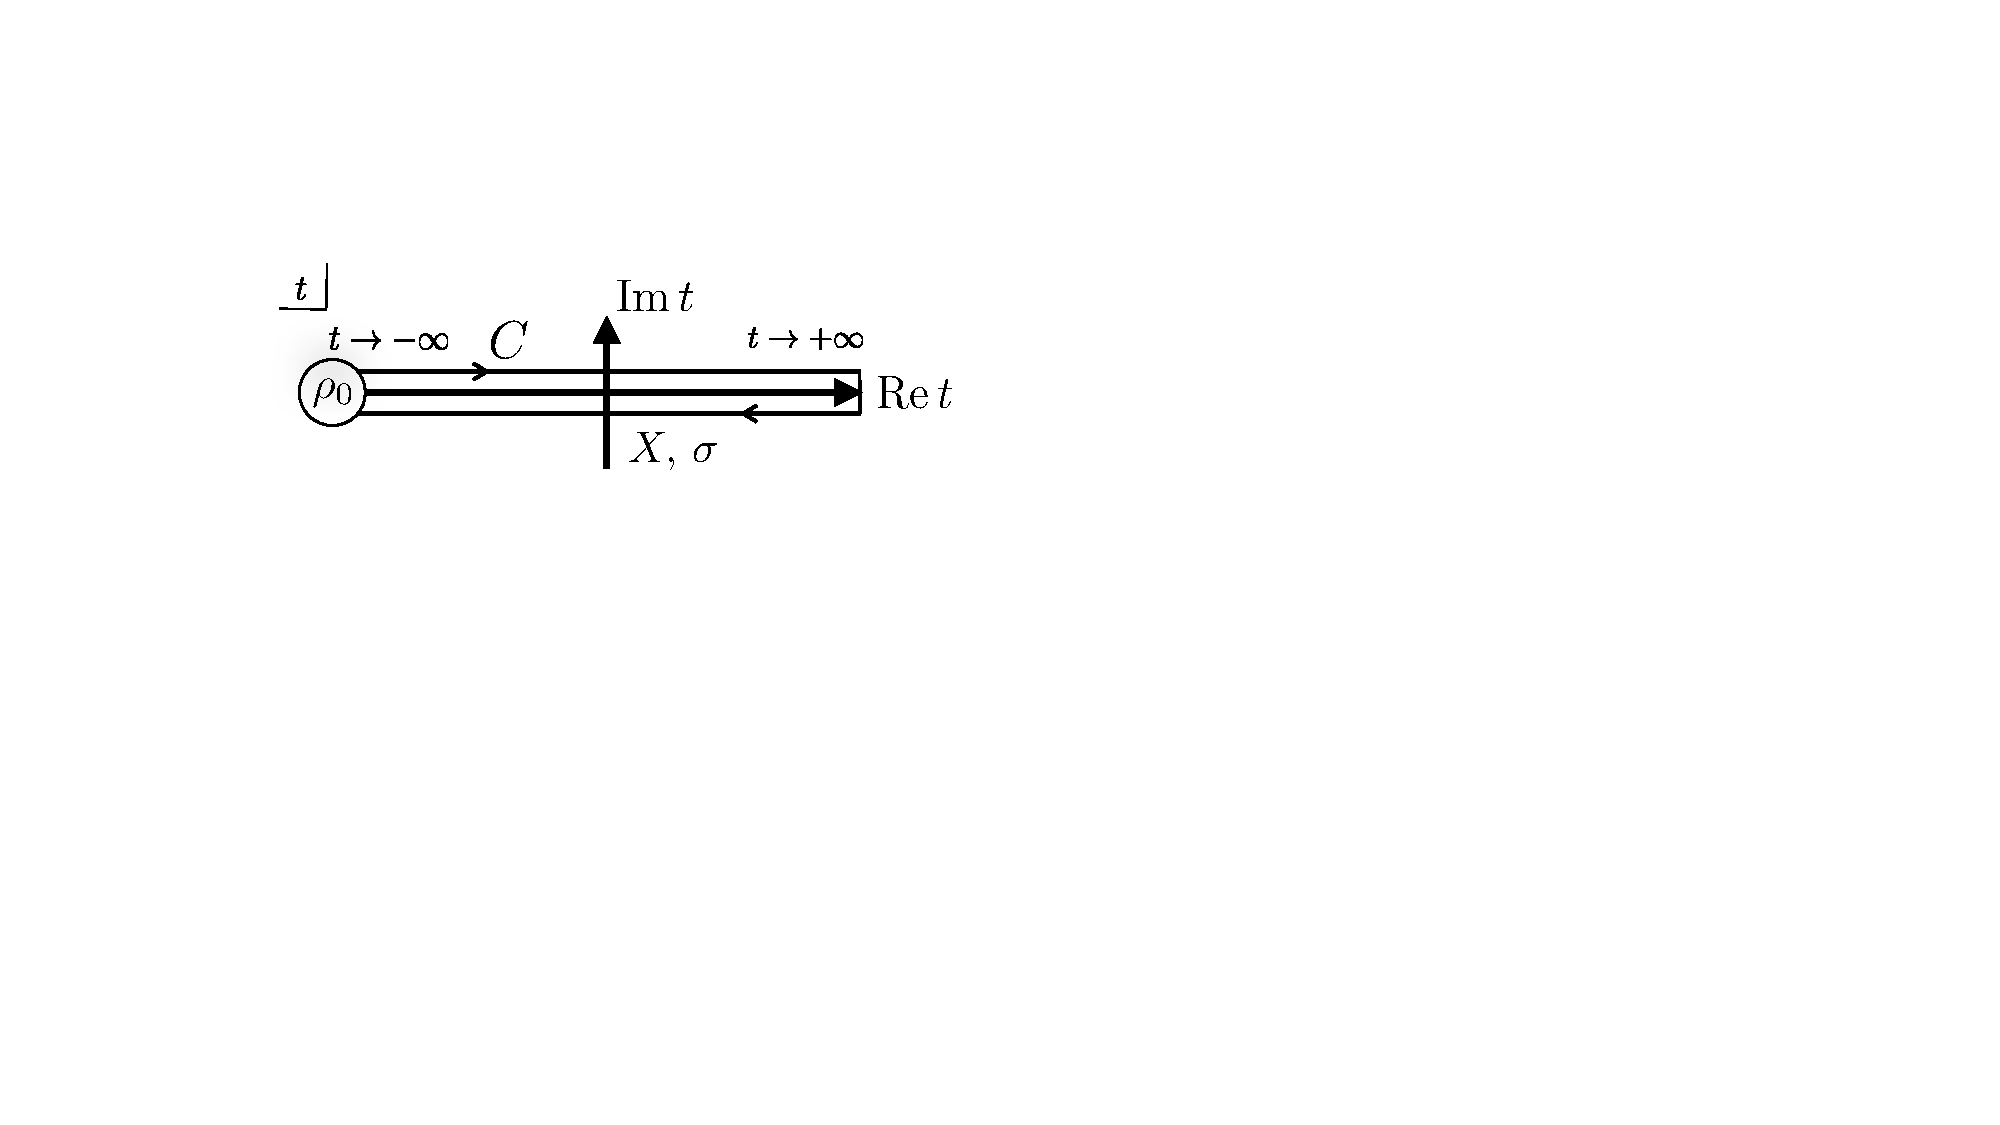
\includegraphics[width=8cm]{original/fig_ctp_x}
\caption{
生成汎関数が定義される閉時間経路。
初期密度演算子 $\hat{\rho}_0$ が熱的密度演算子 $\hat{\rho}_0 \propto e^{-\beta \hat{H}}$ で与えられると仮定すると、負の虚時間方向へ延びる別の経路が存在する（付録\ref{kim}を参照）。}
 
\label{fig:CTP}
\end{center}
\end{figure}


\medskip
微視的作用 $S_{\rm micro}$ が時間並進対称性を持つとき、式\eqref{pi_micro}の指数部は、$\epsilon_a~(a=1,2)$ でラベル付けされる二重化された時間並進\footnote{
正確には、$\epsilon_1\neq\epsilon_2$ の変換は、先に述べた $1$ と $2$ の変数間の $\mathcal{O}(\epsilon)$ の混合によって破られる。ここで、添字 $a=1,2$ の付かない $\epsilon$ は、$i\epsilon$ 処方の無限小パラメータである。}の下で不変である。
\begin{align}
 X_1(t) \to X'_1 (t) = X_1 (t+\epsilon_1)
 \,,
 \quad
 X_2(t)\to X'_2 (t) = X_2 (t+\epsilon_2)
\end{align}
$\sigma_a$ と $J_a$ にも同様の変換則がある。これは、$a=1$ の変数と $a=2$ の変数が分離しているためである。
以下で詳しく述べるように、これら二つの対称性の組合せが、前小節で述べた $\hat{H}_{R}$ と $\hat{H}_A$ に伴う二つの対称性になる。
次に、環境 $\sigma$ を積分消去すると、この対称性構造がどのように変化するかを議論する。
ここで重要なのは、$\sigma_1$ と $\sigma_2$ の間に、オンシェル粒子の生成に関連する非自明な相関が存在するという点である。
その結果、Brown粒子 $X_a$ が環境に結合していると、$\sigma_a$ を積分消去した後の有効作用は、$a=1$ の部分と $a=2$ の部分に分離できない。
\begin{align}
 Z[J_1,J_2]=\int \mathcal{D} X_1 \mathcal{D} X_2 
 \exp \Big[iS_{\rm eff}[X_1,X_2;J_1,J_2] \Big]
 \,.\label{eq:MSR10}
\end{align}

\begin{figure}[t]
 \begin{center}
  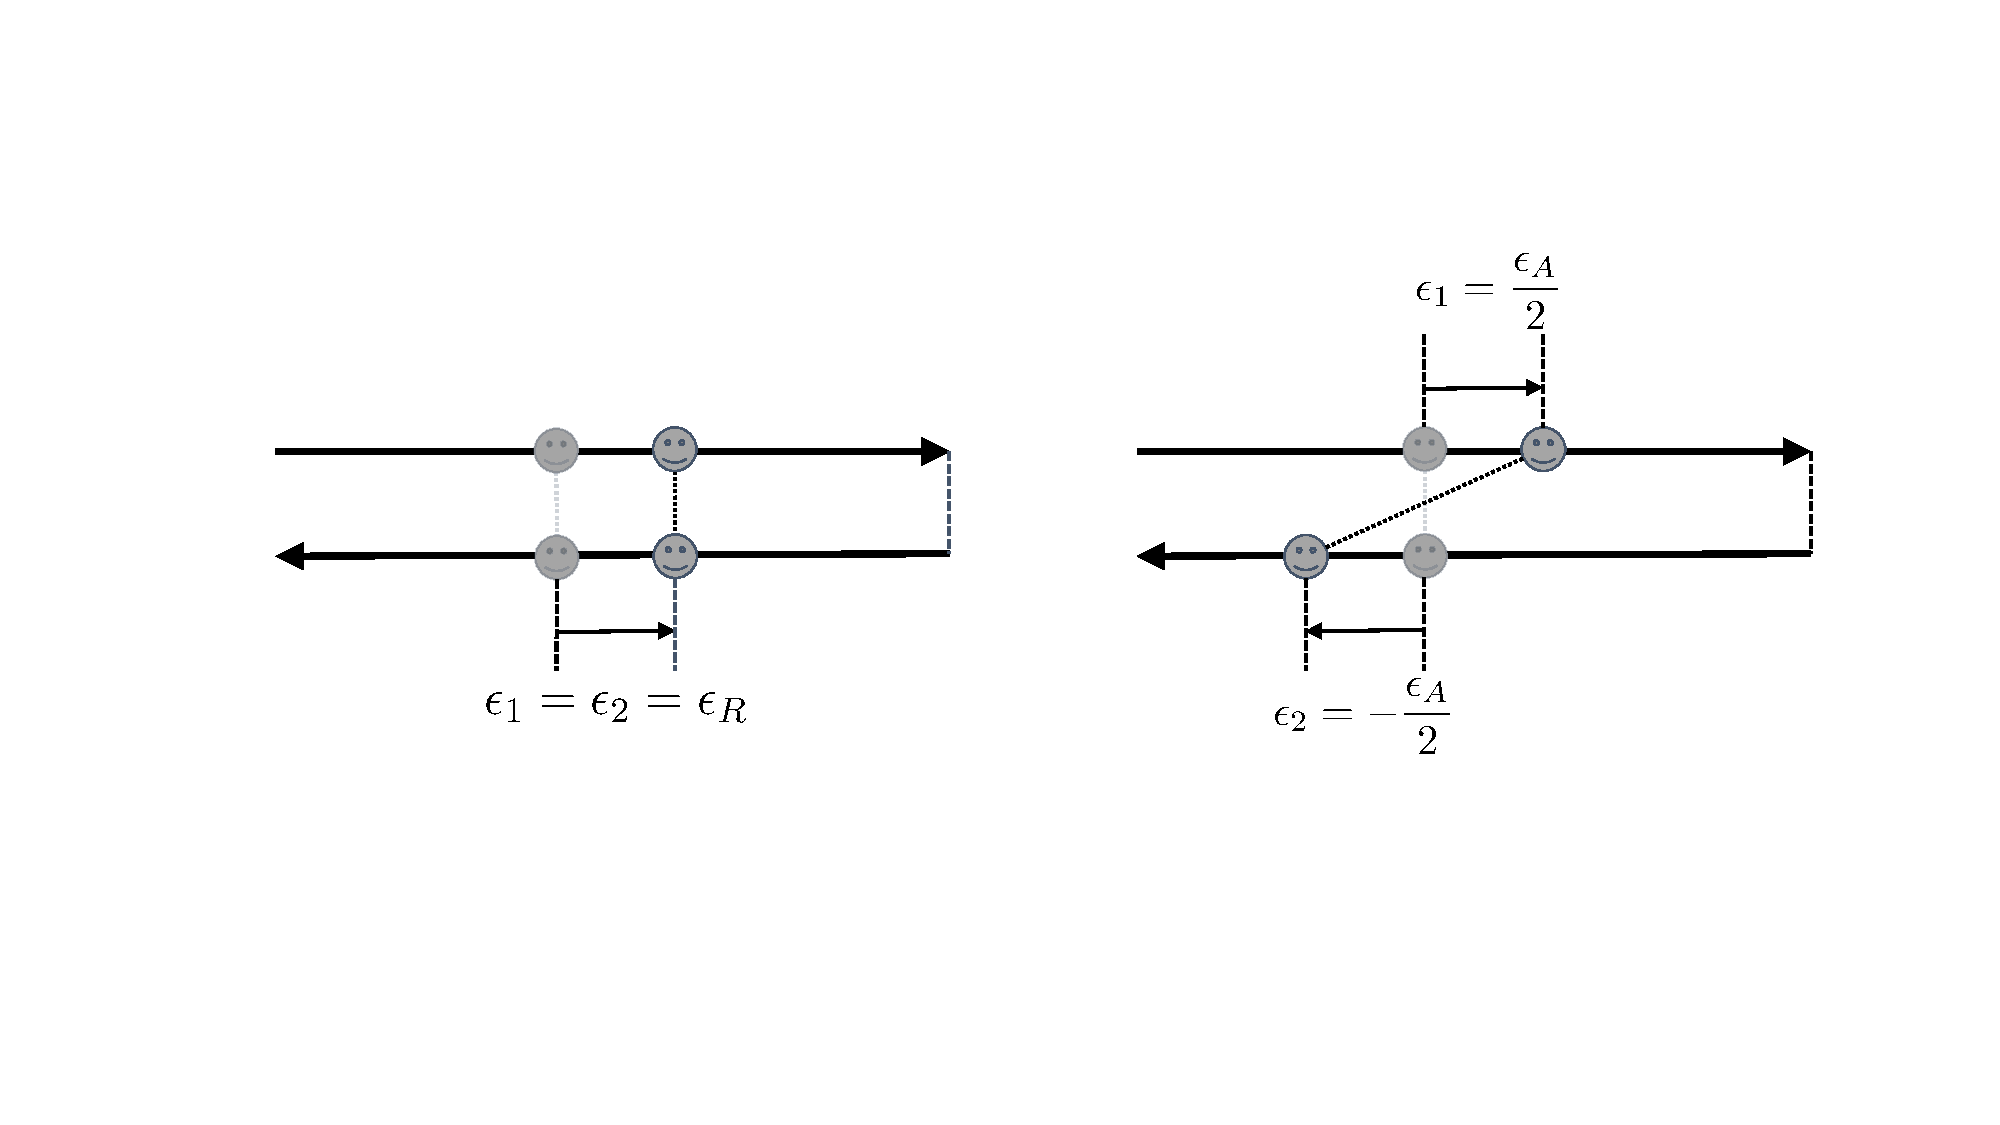
\includegraphics[width=15cm]{original/fig_eRA}
  \caption{
閉時間経路上の $\epsilon_{R}$ 変換と $\epsilon_{A}$ 変換。
$\epsilon_{R}$ は $a=1,2$ の変数を同じ方向に並進させる一方、$\epsilon_{A}$ は逆方向に並進させる。
$t$ に陽に依存しない Lagrangian は、$\epsilon_{R}$ 並進の下でのみ不変である。
右図に示すように、同時刻の $1$--$2$ 結合は、$\epsilon_A$ 変換を行うと、もはや同時刻の結合ではなくなる。}
  \label{fig:TwoTimeTr}
 \end{center}
\end{figure}


よく知られた具体例を調べ、Brown粒子に対する $S_{\mathrm{eff}}[X_1,X_2]$ を具体的に求めよう。
軽い調和振動子 $\sigma (t) =\{x_1 (t), \cdots, x_N(t)\}$ と結合した一次元の Brown点粒子 $X(t)$ を考える。その全作用は、次式で与えられる。
\begin{equation}
 S_{\mathrm{total}}[X,\{x_n\}] 
  = \int dt 
  \Big[ L_{\mathrm{sys}} + L_{\mathrm{env}} + L_{\mathrm{int}} \Big] .
  \label{eq:TotalL}
\end{equation}
ここで、$L_{\mathrm{sys}},\, L_{\mathrm{env}}$ および $L_{\mathrm{int}}$ は、それぞれ Brown粒子、環境の調和振動子、およびそれらの相互作用に対する Lagrangian を表す。
\begin{equation}
 L_{\mathrm{sys}} 
  = \dfrac{M}{2} \dot{X}^2 - V (X), 
  \quad
  L_{\mathrm{env}} 
  =  \displaystyle{\sum_{n=1}^N }
  \left[ \dfrac{m_n}{2} \dot{x}_n^2 - \dfrac{1}{2} m_n \omega_n^2 x_n^2 \right], 
  \quad
  L_{\mathrm{int}} 
  =  \displaystyle{\sum_{n=1}^N} g_nx_n X , 
  \label{eq:EachL}
\end{equation}
$m_n$ と $\omega_n$ は、それぞれ環境の第 $n$ 調和振動子の質量と振動数である。
簡単のため、$X$ と $x_n$ の間には、結合定数 $g_n$ を持つ線形結合を導入した。
環境には、いわゆる\textit{Ohmic 浴}~\cite{kamenev2011field}を用いる。これは連続スペクトルを持つので、$N$ は非常に大きい（詳細は付録\ref{kim}を参照）。
また、初期時刻（$t=-\infty$）では熱平衡にあると仮定する。
付録\ref{kim}では、この Lagrangian から出発して、重い粒子に対する次の有効作用を導出する。
\begin{align}
 iS_{\mathrm{eff}} [X_1,X_2] 
 = i\int dt\, 
 &\left[ - \frac{M}{2} X_{i} D^{-1}_{ij} X_{j} - V(X_1) + V(X_2) \right], 
 \label{eq:MSR3}
\end{align}
ここで、次のように定義した。
\begin{align}
 D^{-1}_{ij}
 = \begin{pmatrix}
    \partial_{t}^{2}-\dfrac{iA}{M} & \gamma\partial_{t} + \dfrac{iA}{M} 
    \vspace{5pt} \\
    - \gamma\partial_{t} + \dfrac{iA}{M} & - \partial_{t}^{2} - \dfrac{iA}{M}
   \end{pmatrix}
   \quad
   {\rm with}
   \quad
   A=2M\gamma/\beta
   .
  \label{D-1}
\end{align}
ここで、$\gamma$（$>0$）は、Ohmic 浴における調和振動子の振動数分布を特徴付けるパラメータである。
熱平衡を仮定したため、FDR $A=2M\gamma/\beta$ が満たされていることに注意しよう。
予想したとおり、環境 $x_n$ を積分消去すると混合項が生じ、$a=1,2$ の変数は互いに結合する。
この混合項により、有効作用は $\epsilon_1 \neq \epsilon_2$ という選択の下では、もはや不変ではない。
したがって、有効作用の対称性は、次のようにパラメータを制限した時間並進対称性となる（図\ref{fig:TwoTimeTr}の左図を参照）。
\begin{align}
\label{eR}
 \epsilon_1 = \epsilon_2 = \epsilon_R 
 \,,
\end{align}
ここで、共通のパラメータを $\epsilon_R$ と表した。
また、後で用いるため、（陽に）破れた対称性も $\epsilon_A$ を用いて次のように表す（図\ref{fig:TwoTimeTr}の右図を参照）。
\begin{align}
\label{eA}
 \epsilon_1 = - \epsilon_2 = \frac{\epsilon_A}{2} \,.
\end{align}
このように、ゆらぎと散逸が存在すると、微視的作用の二つの時間並進対称性は、対角的な対称性 $\epsilon_1=\epsilon_2$ へと破れる。
これは、まさに前小節で見たことである。



\medskip
前小節の議論との関係をより明確に見るには、次の新しい基底を導入すると便利である。
\begin{align}
 X_R = \frac{X_1 + X_2}{2}\,,
 \quad
 X_A= X_1 - X_2  \,.
\end{align}
$\epsilon_R$ をパラメータとする変換\eqref{eR}の下で、これらは次のように変換する。
\begin{align}
 \begin{cases}
  X_R(t) \to X'_R (t) = X_R (t+\epsilon_R)\,, \\
  X_A(t) \to X'_A(t) = X_A (t+\epsilon_R)\,,
 \end{cases}
\end{align}
$X_{R}$ と $X_A$ を MSR 形式の同名の変数と同一視すると、これはまさに、Fokker-Planck Hamiltonian が生成する $H_A$ 変換\eqref{eq:Timetr1}である。
一方、$\epsilon_A$ をパラメータとする、陽に破れた変換\eqref{eA}は、次の形を取る。
\begin{equation}
  \begin{cases}
   X_R(t) 
   \to X'_{R}(t) 
   = X_R(t)+ \dfrac{1}{4} \epsilon_A \dot{X}_A(t) + O (\epsilon_A^2) \,,
   \vspace{5pt} \\
   X_A(t) 
   \to X'_A(t) 
   = X_A(t) +\epsilon_A\dot{X}_R+ O (\epsilon_A^2)\,.
  \end{cases}
\end{equation}
ここで、$X_{R} =O (\hbar^0)$ および $X_A = O(\hbar)$ となるように $\hbar$ 依存性を割り当てると便利である。
すると、半古典極限（$\hbar\to0$）において、上の変換は次の形に帰着する。
\begin{equation}
 \begin{cases}
  X_R(t) \to 
  X'_R(t) = X_R(t) + O(\epsilon_A^2)\,,
  \\
  X_A(t)\to 
  X'_A(t) = X_A(t) + \epsilon_A \dot{X}_{R} + O(\epsilon_A^2)\,,
 \end{cases}
\end{equation}
その最低次の部分は、まさに Brown粒子のもとの Hamiltonian が生成する $H_R$ 変換\eqref{eq:Timetr2}である。
これは、MSR 有効作用が Schwinger-Keldysh 作用の半古典極限として得られることを意味する。
\medskip

まとめると、Schwinger-Keldysh 形式における微視的（UV）作用は、閉時間経路という性質のためにすべての場が二重化されるのと同様に、$\epsilon_R$ と $\epsilon_A$ でラベル付けされる二重化された時間並進対称性を持つ。
しかし、環境を積分消去した後の有効（IR）作用には、$a=1,2$ の変数間の混合が含まれ、これは確率的効果および散逸効果と解釈される。
このような混合は、二重化された対称性を、$\epsilon_R$ でラベル付けされる対角的な対称性へと陽に破る。この対称性は、まさに Fokker-Planck Hamiltonian が生成する $H_A$ 時間並進変換である。
一方、$\epsilon_A$ でラベル付けされる陽に破れた対称性は、半古典極限（$\hbar \to 0$）において、Brown粒子の Hamiltonian が生成する $H_R$ 変換と同一視される。
これで、$H_A$ 対称性の自発的破れに基づく有効場理論の観点から、非定常な確率分布を記述する可能性を議論できるようになった。これが、次節で議論する主題である。




